\documentclass{article}
\usepackage{tikz}
\usepackage[margin=2cm]{geometry}

\begin{document}

\begin{center}
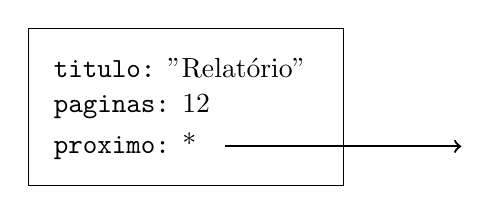
\begin{tikzpicture}

% Caixa exterior
\draw (0, 0) rectangle (4, 2);

% Texto por linha (sem divisórias internas)
\node[anchor=west] at (0.2, 1.5) {\texttt{titulo:} "Relatório"};
\node[anchor=west] at (0.2, 1) {\texttt{paginas:} 12};
\node[anchor=west] at (0.2, 0.5) {\texttt{proximo:} *};

\draw[->, thick] (2.5, 0.5) -- ++(3, 0);


\end{tikzpicture}
\end{center}

\end{document}